\section{Approach and Methodology}
This is a multi-class classification problem with many labeled training examples where the form of the class distributions are not known. This makes supervised discriminative classifiers the most appropriate family of tools. While tree-based methods and support vector machines are viable options, convolutional neural networks (CNNs) are the obvious tool for image-based classification.

\subsection{Learning from Previous Submissions}
Our group did not have expertise in designing and training CNNs before this project. Fortunately, the competition's \textit{Kaggle} community was extremely collaborative and communicative in nature, with many top submissions publishing and discussing their solutions in detail for others to reproduce their results. We began by exploring existing solutions to get an idea of the tools that others found useful and to better understand a variety of approaches used. 

A big takeaway from exploring \textit{Kaggle} was that the Python-based \texttt{pytorch} was clearly the most popular machine learning framework used among submissions, and we decided to develop a \texttt{pytorch}-based solution as well. We also incorporated helper functions that have seemed to have been widely disseminated among solutions; any functions copied from \textit{Kaggle} include a link to the submission from which it was taken. 

\subsection{Image Pre-Processing}
\begin{figure}[htbp]
    \centering
    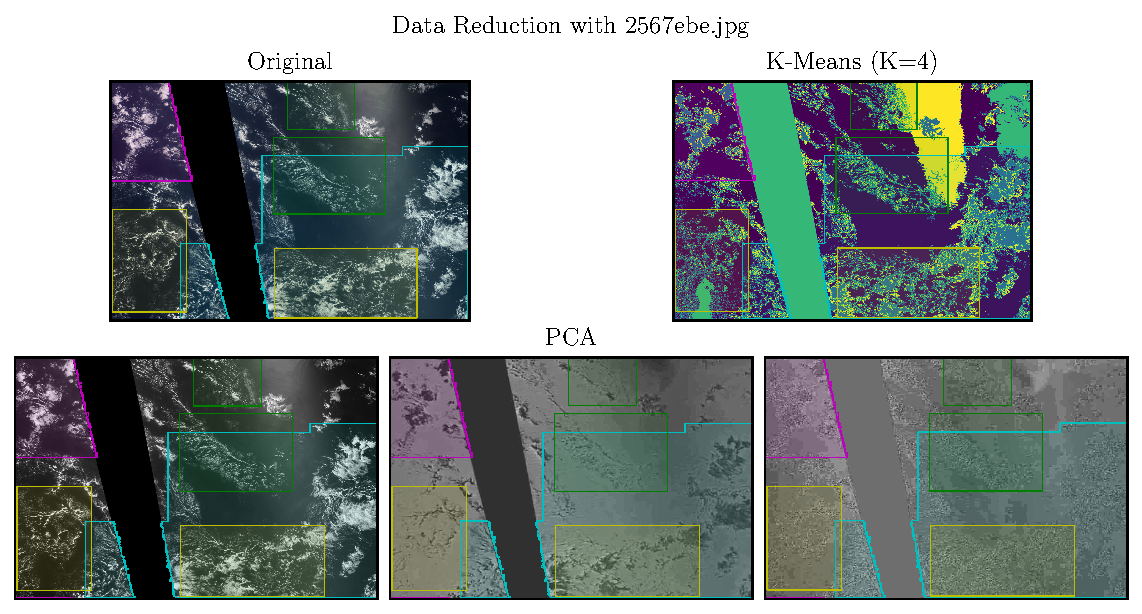
\includegraphics[width=7.5in]{figs/data_redux.pdf}
    \caption{Comparing K-means (top right) and PCA (bottom row) applied to the original full-resolution image containing all four classes (top left). From left to right, the PCA channels are listed from greatest to least eigenvalues.}
    \label{fig:PCA}
\end{figure}
%
With so many choices of hyperparameters and CNN Architecture, it's important for a single model to be trained and evaluated in a reasonable amount of time. The images are relatively large, at \(1400 \times 2100\) pixels per RGB channel. When using the full-channel, full-resolution images as inputs, we found a single training epoch took over 3 hours to complete for even simple CNNs. Most competition entries took a few dozen epochs to complete training, which makes rapid model development infeasible with the full-resolution images. Fortunately, the competition is evaluated on masks of images that are down sampled by a factor of four in each dimension. To decrease training time, we decided to down sample the training images and masks similarly. All masks and images are then zero-padded after down sampling to ensure they are compatible with the kernel sizes used in the neural network. 

Because the images are simply clouds over water, three image channels seemed egregious when a single channel could more concisely capture the cloud/water contrast. We decided to further reduce the three-channel image to a single channel via principal component analysis (PCA). We tried other reduction methods such as K-means, but found glare over water and clouds were often classed similarly, even when a high number of groups were used. After the images underwent PCA then down sampling, simple CNNs had a training epoch time of just \(\sim25\) minutes. \Cref{fig:PCA} shows an example of K-means and PCA applied to one of the full-resolution images. 

\subsection{Neural Network Architecture}
The CNN must take in the two-dimensional images. A single pixel can be a member to multiple classes, so a single mask that outputs one assignment per pixel is not sufficient. Our initial approach involved four different networks, each specializing in one class, but that idea would be blind to between-class correlations. We ultimately developed a single CNN that takes in an image and outputs four 2D binary masks, one for each class. 

A variety of design choices were explored when developing the CNN. The most significant design choices involved the architecture of the network, which includes: 
\begin{itemize}
    \item The number of hidden layers.
    \item The number of fully-connected layers, the number of neurons per fully connected layer, and the choice of activation functions.
    \item The number and kernel size of convolution layers.
    \item The number, method, and kernel size of pooling layers.
    \item The order of layers and ways they are connected.
\end{itemize}
Additionally, there are a variety of design choices to make about how the network is trained, including: 
\begin{itemize}
    \item The type of optimizer and its learning rate.
    \item The loss function. An appropriate loss function should be chosen that matches the type of classification being performed; a binary class problem and an exclusive multiclass problem can utilize different information through different loss functions. 
    \item The number of images to include in a training batch. Because of hardware memory constraints, the training and evaluation data are divided into batches of a certain size, with training and optimization occurring over each batch. A single epoch is completed when all batches are used for training once. 
    \item The number of epochs to train over. This is subjective, it is usually sufficient to continue training until the training loss, validation loss, and the DICE evaluation metric converge. 
\end{itemize}

\subsection{Mask Post-Processing}
\begin{figure}[htbp]
    \centering
    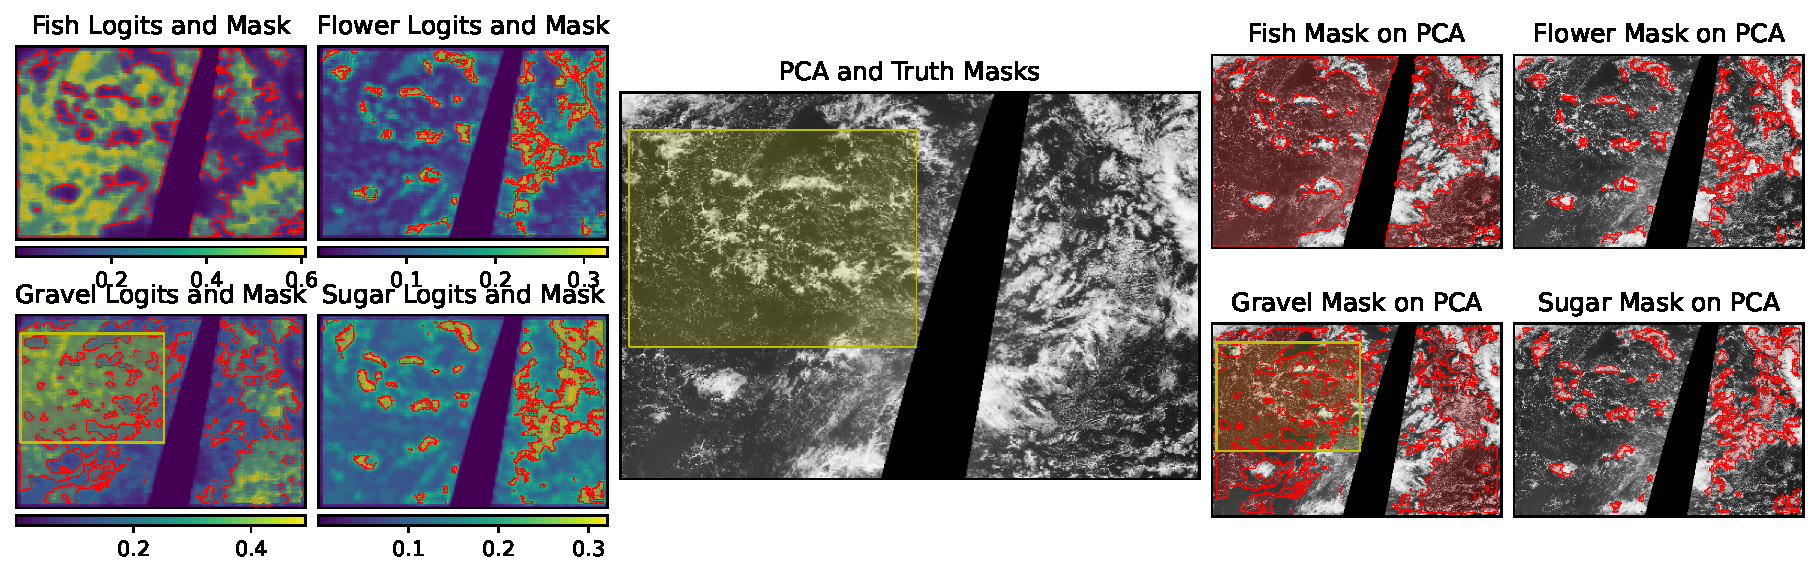
\includegraphics[width=\linewidth]{figs/mask_example.pdf}
    \caption{A figure showing an early model's predicted masks compared to the truth. The center image shows the single-channel PCA image with the truth masks overlaid. The left panels show the logit maps of the image's predicted masks, with the predicted (red) and truth masks overlaid. The right panels show the original PCA image in every panel, with the same predicted and truth masks overlaid to illustrate the features the masks are sensitive to.}
    \label{fig:vis_mask}
\end{figure}
% 
The output of the CNN is four class masks for a given image. These masks are logits, or probabilities that a given pixel has that class membership. \Cref{fig:vis_mask} shows maps of the logits on the left. To translate these logits into binary masks, some thresh holding method must be applied. Unfortunately, the logits can't just be rounded -- even top \textit{Kaggle} entries had logits that didn't usually create good maps through rounding alone. \Cref{fig:vis_mask} masks are created by normalizing the logits for each class across a batch of images, and then rounding. This creates blotchy islands of positive identifications, which is in stark contrast to the rectangle-like masks provided in the training data. 

\begin{figure}[htbp]
    \centering
    \includegraphics[width=\linewidth]{figs/logit_hist.pdf}
    \caption{Distributions of logits and mask values for a batch of images. Each column corresponds to a different class; the first row shows the distribution of logits (log scale on y-axis), the second row shows the distribution of predicted pixel identifications, and the third row shows the distribution of truth pixel identifications.}
    \label{fig:logit_hists}
\end{figure}

\subsection{Additional Ideas}
\begin{itemize}
    \item Additional training data via augmentations 
    \item Playing around with the threshold of logits to convert them into masks 
    \item Dilation and erosion
    \item enforce minimum mask sizes 
\end{itemize}